\subsection{Дизайн фреймворка курса}

В постановке задачи мы написали, что хотим тестировать реализацию распределенных сервисов. Чтобы такое тестирование было возможным, мы реализуем сервисы в специальном фреймворке (рис.~\ref{fig:runtime}).

\begin{figure}[h]
    \centering
    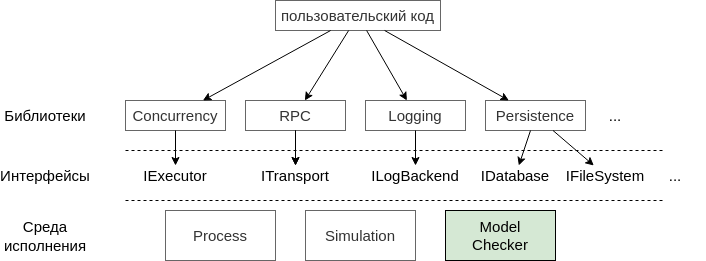
\includegraphics[width=\textwidth]{img/runtime.png}
    \caption{Дизайн фреймворка курса}
    \label{fig:runtime}
\end{figure}

В фреймворке выделяются три уровня:

\begin{enumerate}
    \item Уровень приложения, в котором пользователь описывает свои сервисы с помощью богатого набора высокоуровневых инструментов:
    \begin{itemize}
        \item Отказоустойчивый RPC 
        \item Concurrency (stackful fibers, futures, cancellation)
        \item Инструменты observability: логирование и распределенная трассировка
        \item Persistence (база данных, write-ahead логи, файловая система)
    \end{itemize}
    
    \item Все эти компоненты опираются на небольшой набор базовых абстракций:
    \begin{itemize}
        \item RPC опирается на ITransport – асинхронную шину сообщений для коммуникации между узлами
        \item Concurrency опирается на интерфейс IExecutor – планировщик, исполняющий короткие неблокирующие задачи
        \item Persistence – на интерфейсы IDatabase (локальное KV хранилище) и IFileSystem
        \item и т.п.
    \end{itemize}
    
    \item За реализацию этих интерфейсов отвечает самый низкий уровень – \emph{среда исполнения}.
\end{enumerate}

Среда исполнения, таким образом, отделена от реализации конкретных систем / алгоритмов слоем простых интерфейсов и заключает в себе весь недетерминизм исполнения. Такой дизайн позволяет без изменения пользовательского кода подменять среду исполнения:
\begin{itemize}
    \item процесс-демон с исполнением в многопоточном work-stealing планировщике задач и транспортом сообщений через протокол TCP.
    \item детерминированная симуляция с внедрением сбоев
    \item та часть, разработке которой посвящена работа, model checker.
\end{itemize}

Таким образом, мы получим фреймворк, который сочетает разные подходы к тестированию: и fault-injection, и model checking.

Model checker – это библиотека, которая должна с одной стороны предоставлять узлам системы среду исполнения (сетевой транспорт, планировщик и т.д.), а с другой – представлять собой инструмент с некоторым перебором состояний этого кода.

Реализацию model checker мы разберем с двух сторон: как реализован перебор состояний теста и как реализована среда исполнения для узла распределенной системы, которую пишет пользователь. 
